\subsection{\emph{Legs Plugin}}
\label{subsec:legsplugin}

\emph{Legs plugin} merupakan \emph{Gazebo plugin} yang digunakan untuk menghubungkan model pengguna dengan sistem komunikasi antar-proses ROS 2.
Seperti yang terlihat pada gambar \ref{fig:integrasipluginpengguna},
  \emph{plugin} ini dibuat agar model pengguna yang ada di simulasi bisa terabstraksi untuk diakses dan dimanipulasi oleh \emph{smart assistive posture device} maupun \emph{dummy node} yang mengirimkan data yang sama dengan yang dikirim oleh \emph{smart assistive posture device}.

\emph{Legs plugin} memiliki dua kegunaan utama.
Yang pertama adalah untuk mengubah posisi dan orientasi dari model pengguna sesuai dengan posisi dan orientasi yang diterima dari perhitungan \emph{smart assistive posture device} maupun \emph{dummy node}.
Sedangkan yang kedua adalah untuk mengubah posisi \emph{joints} di kaki menjadi duduk jongkok maupun berdiri sesuai dengan nilai postur kaki yang dikirim oleh \emph{smart assistive posture device} maupun \emph{dummy node}.

\begin{figure}[ht]
  \centering
  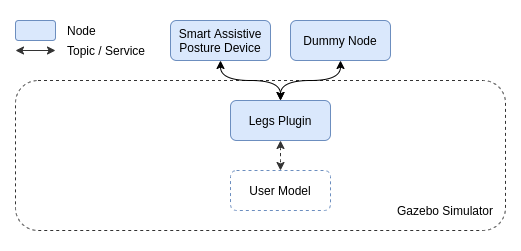
\includegraphics[scale=0.5]{gambar/integrasi-plugin-pengguna.png}
  \caption{Diagram integrasi \emph{plugin} untuk model pengguna di simulasi.}
  \label{fig:integrasipluginpengguna}
\end{figure}

\lstinputlisting[
  language=C++,
  caption={\emph{Class} dari \emph{legs plugin}.},
  label={lst:legsplugin}
]{kode/plugin/legs_plugin.cpp}

Sama seperti \emph{navigation plugin} yang ada di bagian \ref{subsec:navigationplugin},
  seperti yang terlihat pada potongan kode \ref{lst:legsplugin},
  \emph{plugin} ini juga ditulis dalam bahasa C++ dan dibuat dengan menurunkan \emph{class} \lstinline{gazebo::ModelPlugin} sebagai \emph{parent class} dari \emph{class} ini.
\emph{Plugin} ini menggunakan objek \lstinline{beine_cpp::LegsConsumer} yang memudahkan \emph{subscription} dari \emph{topic} yang berhubungan dengan data yang dikirim oleh \emph{smart assistive posture device}.
Data tersebut berupa data posisi yang dikirim melalui \emph{topic} \lstinline{/position},
  data orientasi yang dikirim melalui \emph{topic} \lstinline{/orientation},
  data perintah suara yang dikirim melalui \emph{topic} \lstinline{/command},
  dan data postur kaki yang dikirim melalui \emph{topic} \lstinline{/stance}.

Setelah \emph{plugin} dibuat,
  file SDFormat dari model robot perlu diubah dengan menyematkan \emph{plugin element} di file tersebut.
Seperti yang terlihat pada potongan kode \ref{lst:integrasilegsplugin},
  \emph{plugin element} disematkan sebagai \emph{child element} dari \emph{model element}.
Pada \emph{legs plugin},
  beberapa \emph{child element} lain perlu disematkan pada plugin tersebut,
  seperti \emph{joint force strength element} dan \emph{joint force smoothness element} yang menentukan bagaimana transisi postur kaki terjadi,
  serta \emph{left hip pitch joint element}, \emph{left knee pitch joint element}, dan lain sebagainya yang menentukan \emph{joint element} yang akan diubah ketika terjadi transisi pada postur kaki pengguna.

\lstinputlisting[
  language=XML,
  caption={Integrasi \emph{legs plugin} pada model pengguna.},
  label={lst:integrasilegsplugin}
]{kode/sdf/plugin/legs_plugin.xml}
